\subsection{Aktorbaustein}\label{subsec: Aktorbaustein}
Im folgenden wird die Hardware des Aktorbausteins, ähnlich wie beim Sensorbaustein, beschrieben. Vom Auftraggeber ist ein Aktorbaustein mit 4 Relais, zwei Ausgängen $0..10\;V$ und zwei Eingängen $0..10\;V$ gefordert. Der Aktorbautein wird über 24V-Netzteil mit Spannung versorgt und mithilfe eines On-Off Schalters kann die Spannungsversorgung getrennt werden. Die Logik wird mit 3.3 V betrieben, dazu braucht es ein DC/DC Wandler der die 24 V in 3.3 V wandelt. Die Programmierschnittstelle ist dabei gleich wie beim Sensorbaustein (siehe Kapitel \ref{sec: Sensorbaustein}). Die Spannung der  0...10 V Ausgänge werden über PWM eingestellt und bei den 0...10 V Eingängen kommt der AD-Wandler des Mikrocontrollers zum Einsatz. Damit man weiss welche Relais geschaltet haben, werden LEDs zum Signalisieren verwendet. Um eine bessere Funkreichweite zu erzielen, kann bei dem Aktorbautein, wie beim Sensorbautein, eine Antenne angebracht werden, angedacht ist die Verwendung einer zertifizierten Dipolantenne.

\begin{figure}[h!]
	\centering
	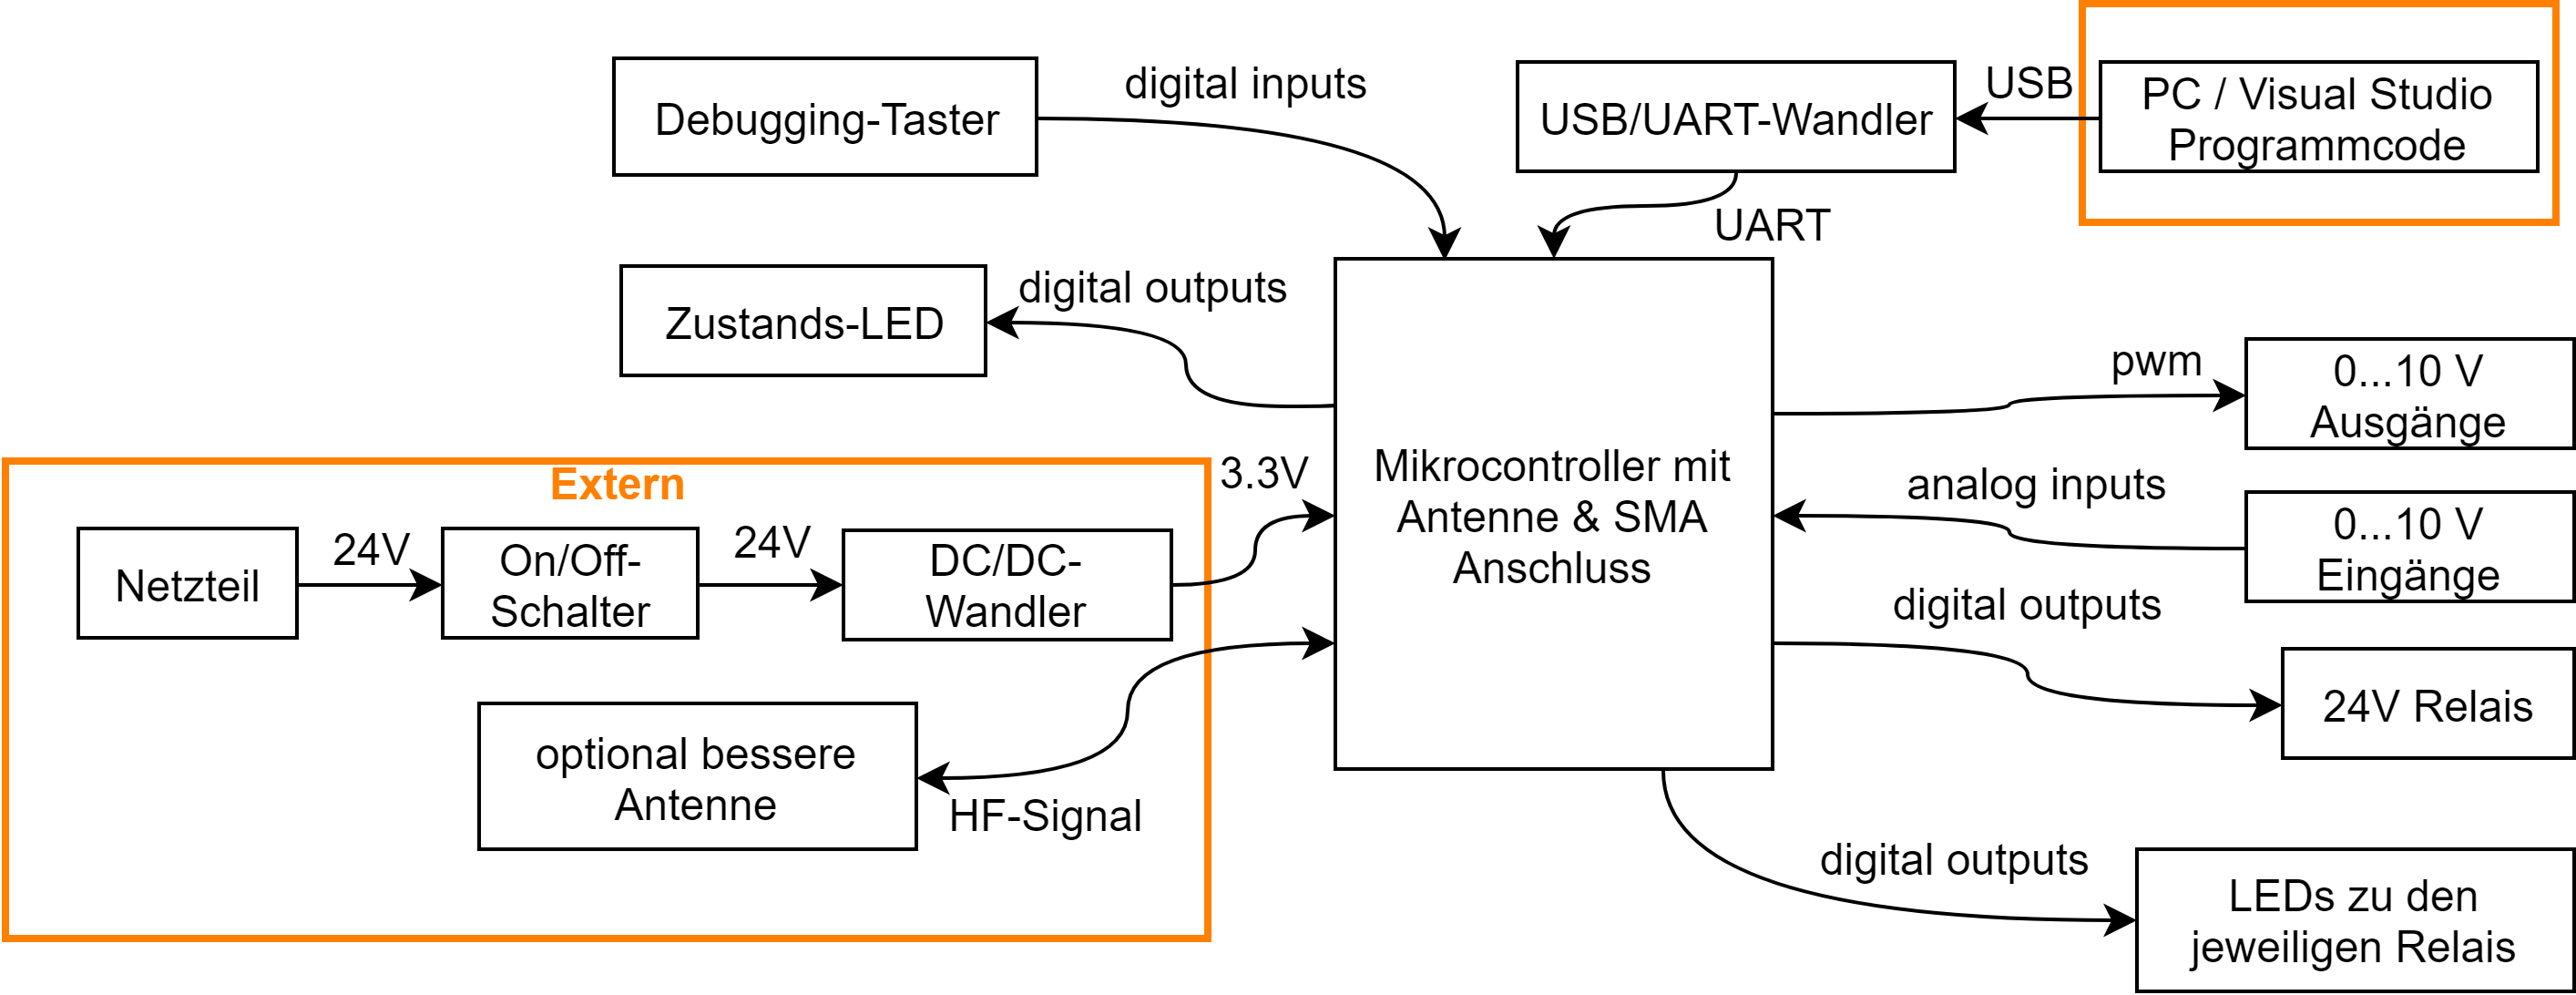
\includegraphics[width=\textwidth]{graphics/Aktorbaustein.png}
	\caption{Übersicht Aktorbaustein}
	\label{pic: Uebersicht_Aktorbaustein}
\end{figure} 

\subsubsection{Mikrocontroller}\label{Hardware Mikrocontroller_Aktor}
Es wird wie schon im Sensorbaustein den ESP32 verwendet, dadurch kann garantiert werden, dass die WiFi-Systeme sich sowohl im Aktor- wie auch im Sensorbaustein sich in etwa gleich verhalten, wodurch der Entwicklungsaufwand minimiert wird. Die vom ESP32 benötigten I/Os werden in der Tabelle \ref{tab: IO Aktorbaustein} aufgelistet und in der Abbildung \ref{pic: ESP32_aktor} erkennt man welche I/Os verwendet wurden. Der Programmieranschluss ist wie beim Sensorbaustein und wird nicht nochmals wiederholt.
\begin{table}[h!]
	\centering
	\begin{tabular}{|l|l|}
		\hline
		\textbf{Name}                      & \textbf{Anzahl} \\ \hline
		digital outputs für Relais \& LED  & 10              \\ \hline
		digital inputs für Buttons         & 3               \\ \hline
		ADC inputs für \glqq $10\;V$\grqq Eingänge  & 2      \\ \hline
		PWM outputs für \glqq$10\;V$\grqq Ausgänge & 2       \\ \hline
		UART Interface für Programmierung  & 3               \\ \hline
	\end{tabular}
	\caption{I/O Aktorbaustein}
	\label{tab: IO Aktorbaustein}
\end{table}
\begin{figure}[h!]
	\centering
	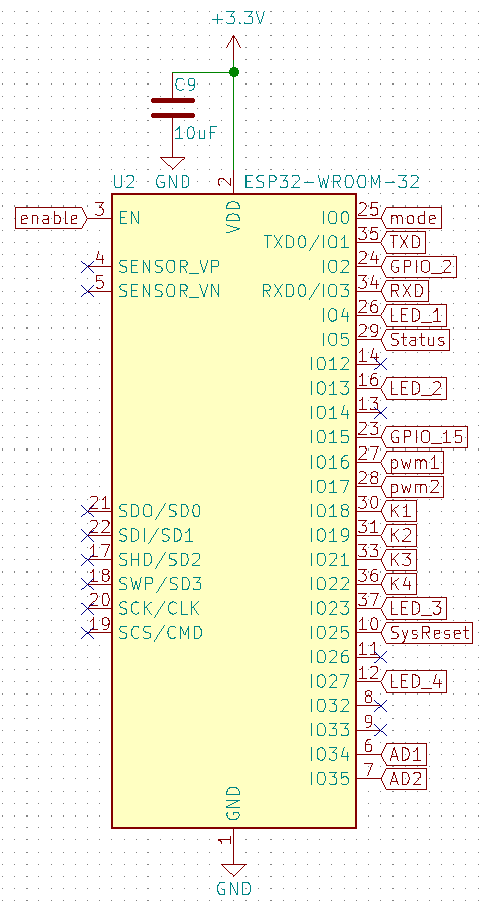
\includegraphics[width=0.45\textwidth]{graphics/shematics_aktor_ESP32.png}
	\caption{Mikrocontroller ESP32 im Aktorbaustein}
	\label{pic: ESP32_aktor}
\end{figure}


\subsubsection{Relais}
Die Anforderungen an ein Relais sind, dass es $230\;V/AC$ schalten und die Relaisspule mit $24\;V/DC$ betrieben werden muss. In der Abbildung \ref{pic: Relais_aktor} ist die Schaltung für ein Relais abgebildet. Als Relais wird ein G5LE-1-VD DC24 von Omron Electronics verwendet, welches mit den oben gennanten Anforderungen kompatibel ist. Der maximale Schaltstrom beträgt 10\,A und die maximale Schaltspannung 250\,VAC oder 125\,VDC. Die Nennspannung der Spule beträgt 24\,VDC, dabei ist garantiert, dass die Spule noch bei 75\,\% also 18\,V der Nennspannung anzieht und bei sicher 10\,\% der Nennspannung also 2.4\,V loslässt. Mit dem Widerstand $R_1$ wird der Einschaltstrom auf $10\;mA$ begrenzt, mithilfe der Freilaufdiode D1 kann die Selbstinduktionsspannung der Spule kurzgeschlossen werden und $R_{24}$ ist ein Pull-Down-Widerstand, so dass der MOSFET sicher sperrt, falls der Output-Pin nicht angesteuert wird \cite{mikrocontroller.net_relais_nodate}. Als MOSFET wird der BSS123 eingesetzt, welcher sich typischerweise schon mit einer Steuerspannung von $1.7\,V$ durchschaltet und eine Drain-Source-Spannung von bis zu $100\,V$ vertragen kann.
\begin{figure}[h!]
	\centering
	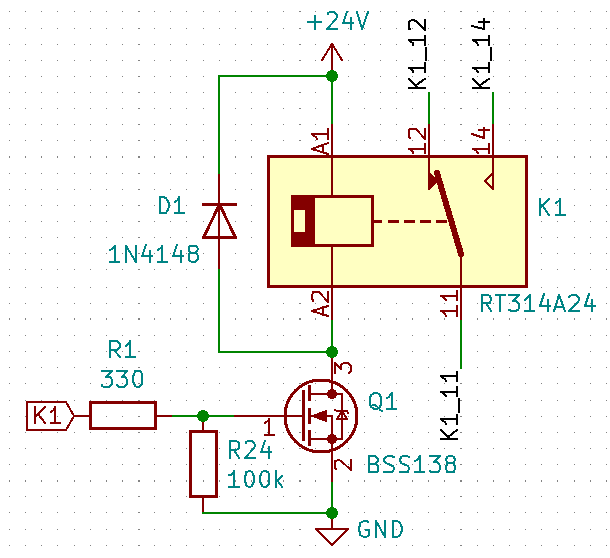
\includegraphics[width=0.45\textwidth]{graphics/shematics_relais.png}
	\caption{Relais im Aktorbaustein}
	\label{pic: Relais_aktor}
\end{figure}

\subsubsection{Eingänge/Ausgänge 0..10 V }
Die $10\;V$ Eingänge werden mittels eines Varistors vor Überspannung geschützt (Abb. \ref{pic: Input_aktor}). Das Signal geht dann durch einen Puffer, damit die Signalquelle nicht belastet wird. Als Verstärker wird hierfür ein LM324A eingesetzt, da er sich gut als rail to rail OpAmp eignet. Als letztes wird mittels einer Spannungsteilers die obere Signalstärke von $10\;V$ auf $ 10\;V \cdot 22/(47+22) = 3.188\;V$ beschränkt. Hier muss dann in der Praxis kalibriert werden, da die Widerstände Toleranz behaftet sind. Bei den $10\;V$ Ausgängen wird jeweils ein PWM vom Mikrocontroller herausgegeben und dann das Signal mittels eines Tiefpasses geglättet (Abb. \ref{pic: Output_aktor}). Die Polfrequenz sowie die $-3dB$ Grenzfrequenz des Tiefpass erster Ordnung berechnet sich für einen 10 Bit AD Wandler und einen Quarz von $40\;MHz$, welcher im ESP32 verbaut ist, folgendermassen: $40\;MHz$ Takt --> $40\;kHz$ PWM --> Zeitkonstante $\tau = 1000/40\;kHz = 25\;ms $ --> Zeit bis zum Endwert $ t_{end}=\tau * ln(1024) = 173\;ms$ --> Grenzfrequenz $f_g = 1/\tau = 40\;Hz$. Die Verzögerungszeit $t_{end}$ ist im Übrigen gleich der Dauer bis die Spannung am Kondensator im Bereich von 1 LSB vom Endwert ist \cite{ronald_locher_2017}. $173\;ms$ Verzögerungszeit scheinen recht lange zu sein, wenn man diese Zeit verkürzen möchte, könnte man auf einen 8 Bit AD Wandler wechseln, wodurch die Polfrequenz auf $156\;kHz$ angehoben wird. Ein anderer Trick besteht darin eine höhere Filterordnung zu wählen. Um eine Abschwächung von 1024 oder 60 dB des $40\;kHz$ PWM Taktes zu erzielen, kann bei zweiter Filterordnung, welche $40\;dB/dec$ Dämpfung hat, die $40\;kHz$ nicht durch 3 Dekaden (Faktor 1000) sondern nur um 1.5 Dekaden (Faktor 31,6) teilen, um die neue Polfrequenz $f_p$ herauszufinden. Hier macht es aber auch Sinn $-80\;dB$ (Faktor 100) bei $40\;KHz$ zu nehmen, um noch ein sauberes Ausgangssignal zu kriegen. Also ist die gewählte Polfrequenz $f_p$ bei $400\;Hz$, $\tau$ bei $2.5\;ms$ und $ t_{end}$ bei $17\;ms$. Die Komponenten der Filterstufen wurden dann wie folgt gewählt: erste Stufe mit $R_1 = 3.9\;k \Omega $ \& $C_1 = 100\;nF$ und die zweite Stufe mit $R_2 = 39\;k \Omega $ \& $C_2 = 10\;nF$. Da $R_1 \cdot C_1 = R_2 \cdot C_2$ ist, ist die Polgüte $q_p = 0.5$, woraus resultiert, dass die Dämpfung bei der Polfrequenz $f_p = 400\;Hz$ einen Wert von $-6\;dB$ annimmt. Die $-3\;dB$ Grenzfrequenz ist folglich bei $f_g = f_p \cdot \sqrt{2^{1/2}-1} = 257\;Hz$ \cite{miller_rc-glied_nodate} und die Dämpfung bei $40\;kHz$ entspricht nach wie vor den gewünschten $-80\;dB$. Nach dem Tiefpass gelangt das Signal in einen positiven Verstärker welcher die maximale Ausgangsspannung des ESP32 von $3.3\;V$ auf theoretisch $ 3.3\;V \cdot (1+ 22/10) = 10.56\;V$ erhöht. An dieser Stelle muss auch wieder kalibriert werden, so dass die maximale Ausgangsspannung $10\;V$ beträgt.
\begin{figure}[h!]
	\centering
	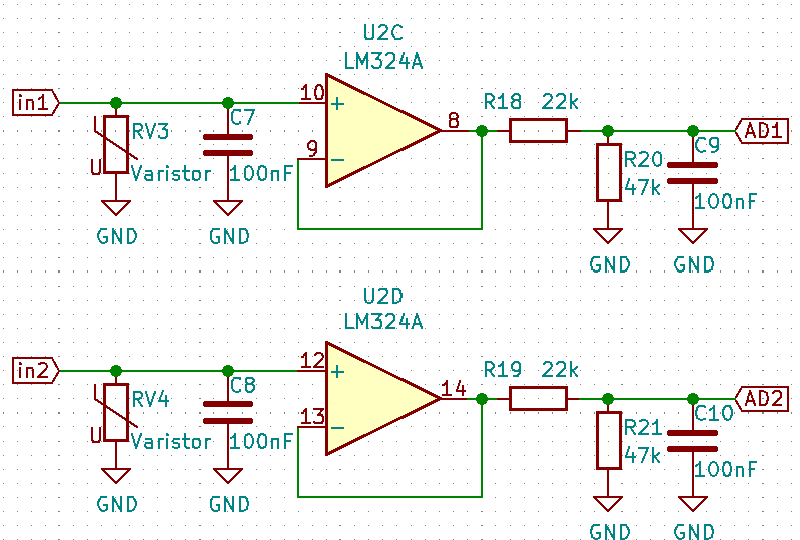
\includegraphics[width=0.55\textwidth]{graphics/shematics_aktor_input.png}
	\caption{Eingänge 10 V Aktorbaustein}
	\label{pic: Input_aktor}
\end{figure}
\begin{figure}[h!]
	\centering
	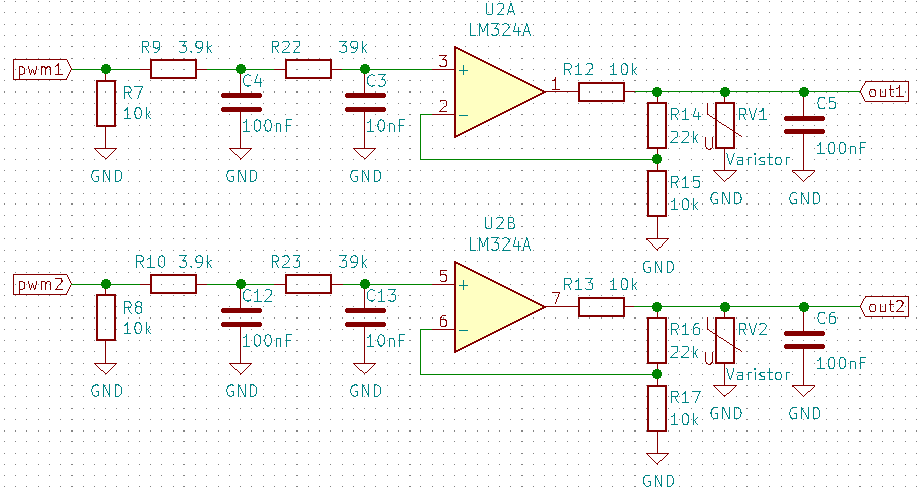
\includegraphics[width=0.8\textwidth]{graphics/shematics_aktor_output.png}
	\caption{Ausgänge 10 V Aktorbaustein}
	\label{pic: Output_aktor}
\end{figure}
\newpage
\subsubsection{Spannungsversorgung}
Mithilfe eines üblichen $24\;V$ Netzgerätes, welches einen Zylinderstecker 2.1 x 5.5 $mm$ (engl. DC Barrel Jack) hat, kann der Aktorbaustein betrieben werden. So gibt z.B von XP-Power ein $18\;W$  $24\;V/DC$ Netzgerät für 11.73 CHF bei mouser. Um die Logik zu betreiben werden jedoch $3.3\;V$ benötigt. Hier kommt der Spannungswandler MIC4680 zum Einsatz, welcher eine Effizienz von bis zu 90 \% aufweist. Vom Wandler Ausgegeben werden typischerweise $3.3\;V$, im aller schlimmsten Fall kann die Spannung jedoch zwischen $3.201\;V$ und $3.399\;V$ liegen. In der Abbildung \ref{pic: Versorgung_aktor} ist das Schema der $3.3\;V$ Spannungsversorgung zu erkennen, es wurde hier noch eine Sicherung eingebaut da der Print nicht zerstört wird, falls zu viel Strom fliesst. Der Schraubklemmen sind dafür da, um z.B einen ON-OFF-Wippschalter, welcher am Gehäuse montiert wird, anzuschliessen. Die Beschaltung um den Spannungswandler ist dem Datenblatt des MIC4680 zu entnehmen.
\begin{figure}[h!]
	\centering
	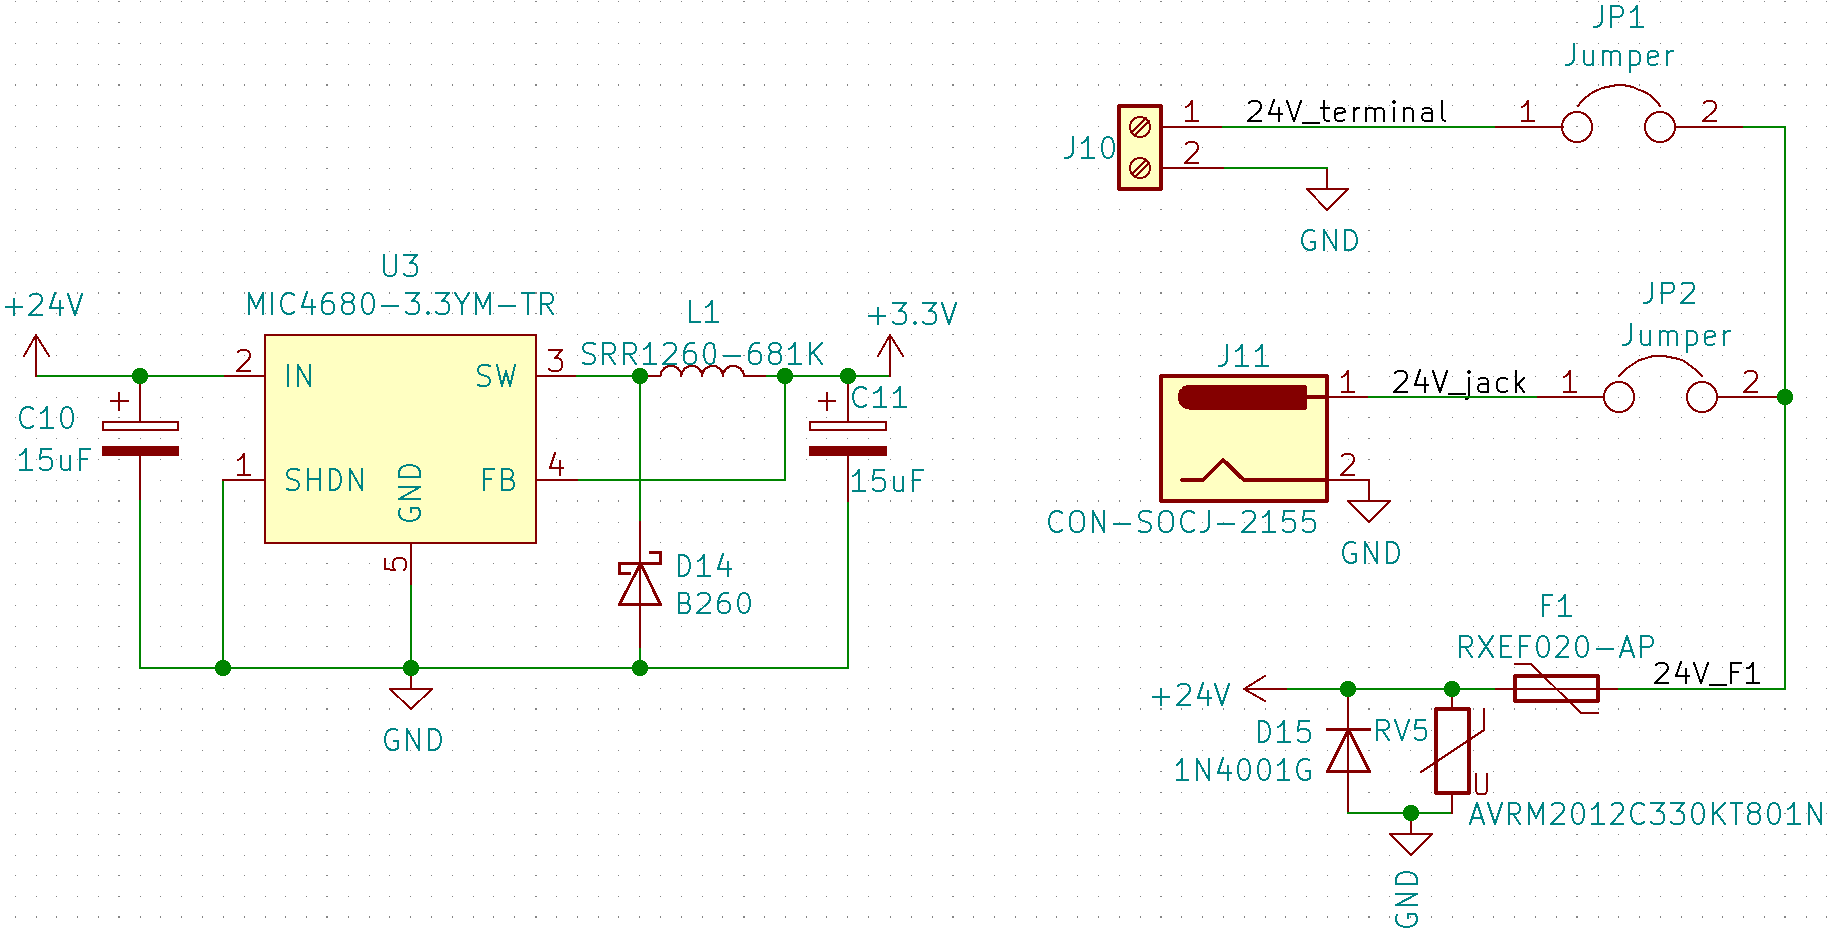
\includegraphics[width=0.7\textwidth]{graphics/shematics_aktor_33V.png}
	\caption{Spannungsversorgung Aktorbaustein}
	\label{pic: Versorgung_aktor}
\end{figure}
\newpage
\subsubsection{Interface}
Die Ausgänge der Relais sowie die 10 $V$ Ein- und Ausgänge sind auf Schraubklemmen geführt (Abb. \ref{pic: Klemmen_aktor}). Es stehen insgesamt 6 LEDs zur Verfügung (Abb. \ref{pic: Buttons_LEDs_aktor}). Die LEDs 1 bis 4 zeigen an ob das jeweilige Relais geschaltet hat. LED5 kann als Status LED verwendet werden. Die Buttons sind die gleichen wie im Sensorbaustein unter Punkt \ref{par: Programmieranschluss} Programmieranschluss.
\begin{figure}[htb]
	\centering
	\begin{minipage}[t]{0.45\linewidth}
	\centering
	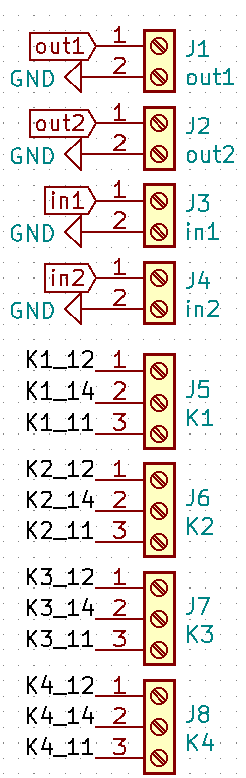
\includegraphics[width=0.35\textwidth]{graphics/shematics_aktor_klemmen.png}
	\caption{Klemmenanschlüsse Aktorbaustein}
	\label{pic: Klemmen_aktor}
	\end{minipage}% <- sonst wird hier ein Leerzeichen eingefügt
	\hfill
	\begin{minipage}[t]{0.45\linewidth}
	\centering
	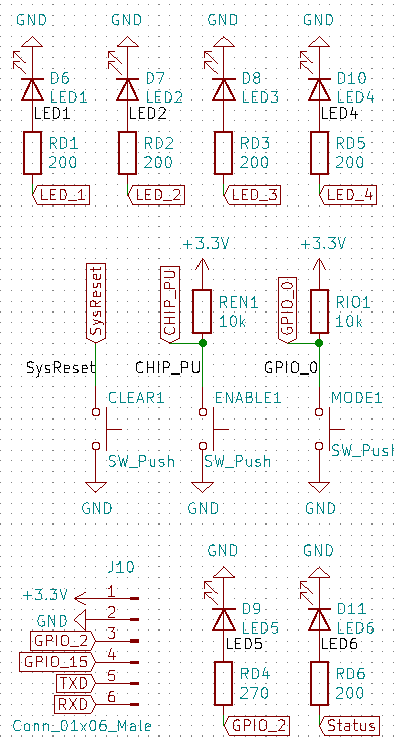
\includegraphics[width=0.9\textwidth]{graphics/shematics_aktor_buttons_LEDs.png}
	\caption{Buttons und LEDs Aktorbaustein}
	\label{pic: Buttons_LEDs_aktor}
	\end{minipage}
\end{figure}

